\chapter{Techno-economic Analysis}
This section discusses the technical and economic aspects and impacts of the project. It covers time management, the project budget, technical impact, return on investment, and the project's potential for commercialisation.
\section{Planning and Time Management}
\begin{figure}[H]
    \centering
    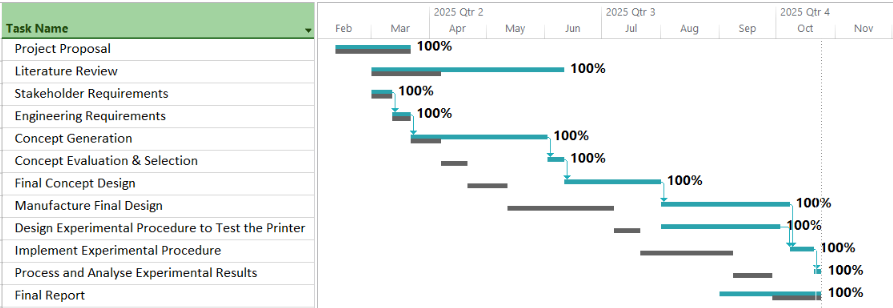
\includegraphics[width=\textwidth]{figs/ProjectGanttChart.png}
    \caption{Project Gantt Chart}
    \label{fig:gantt}
\end{figure}
The Gantt chart in Figure~\ref{fig:gantt} compares the predicted baseline duration (grey) of each project activity with the actual timeline (blue) in which the tasks were completed. It can be seen that the literature review extended over a significantly longer period than initially planned, due to the high workload from other modules during the first semester. A second major deviation occurred during the concept generation phase, which exceeded its planned duration because of an overly optimistic initial time estimate. The remaining project activities -- including completing the design process, manufacturing, assembling, and conducting the experimental work -- had to be completed within a shorter time frame to meet the final project deadline of 24~October~2025.

\section{Budget}
\begin{table}[H]
    \centering
    \caption{Estimated Project Budget}
    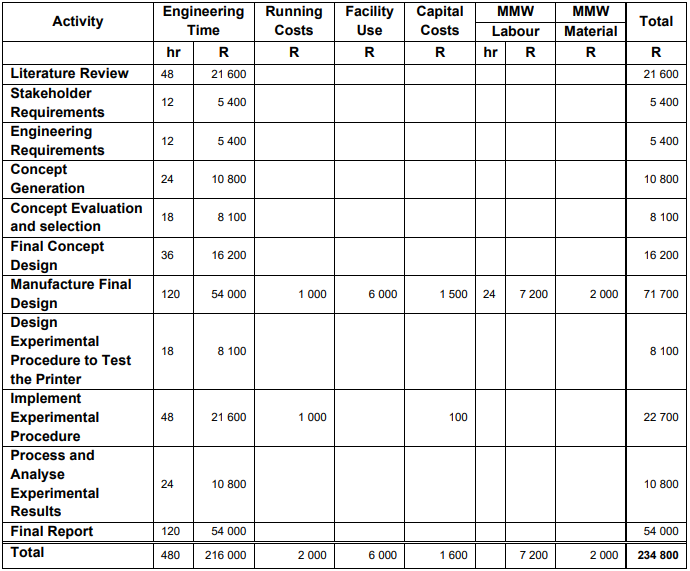
\includegraphics[width=0.8\textwidth]{figs/TheoreticalBudget.png}
    \label{tab:theoreticalBud}
\end{table}
\begin{table}[H]
    \centering
    \caption{Actual Project Cost}
    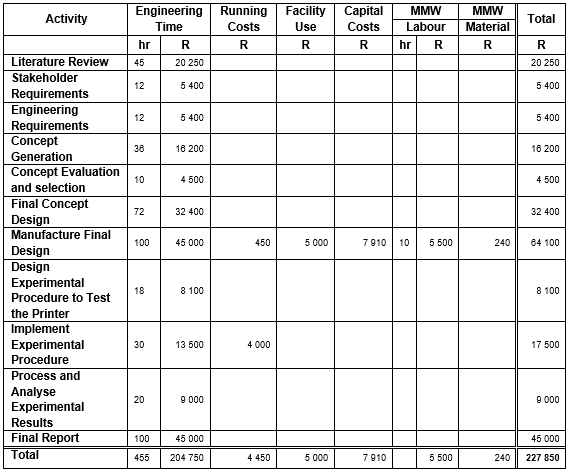
\includegraphics[width=0.8\textwidth]{figs/Actual Costs.png}
    \label{tab:actualCost}
\end{table}
The predicted budget and estimated final costs are shown in Tables~\ref{tab:theoreticalBud} and~\ref{tab:actualCost}. The actual cost of R227 850 was slightly below the initially predicted budget of R234 800. The largest discrepancies between the planned and actual expenses occurred in the running, capital, and workshop cost categories. These differences occurred because the final design was completed after the proposed budget had been estimated. Therefore, many required components that needed to be purchased or manufactured were not yet identified. In addition, the running cost estimate did not accurately account for electricity consumption and unplanned consumables such as lubricant.

The cost of component procurement, whether manufactured by the university or externally sourced, is summarised in Table~\ref{tab:costs}. This table reflects the total cost of developing the complete prototype, excluding the engineering time required for the system design.
\begin{table}[H]
    \centering
    \caption{Prototype Costs}
    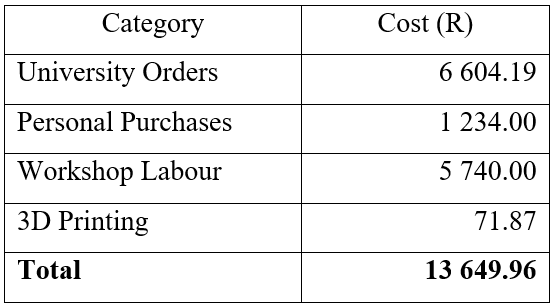
\includegraphics[width=0.5\textwidth]{figs/Costs.png}
    \label{tab:costs}
\end{table}

\section{Technical Impact}
The development of the hydrogel 3D printer provides a meaningful technical contribution to biomedical and tissue engineering research. The project demonstrates that repeatable hydrogel extrusion can be achieved using a cost-effective bioprinting system. On a technical level, the functional prototype serves as a flexible research tool for studying flow behaviour of unknown hydrogels. Building on the first iteration of this project -- done in 2024 -- this prototype integrates embedded control, modular hardware, and tunable parameters. It has also lowered the cost barrier for local tissue engineering research and established a stronger foundation for continued bioprinter development within the university.
\section{Return on Investment}
The time and money that was invested into this project resulted in a functional research platform. In the short term, the bioprinter serves as a means of characterising different unknown gels. In the long term, the system offers a low-cost alternative to imported high-cost bioprinters. Further development of this project by future students can refine the prototype into a laboratory-grade bioprinter with temperature control and closed-loop pressure feedback. The project therefore provides a high return on investment through its affordability, adaptability, and potential use as a research tool.
\section{Potential for Commercialization}
The project outcome is a functional prototype of a hydrogel 3D printer that shows potential for commercialization as an affordable and modular bioprinter for research institutions. Current commercial bioprinters, like the BIO X series, are not accessible for many laboratories due to their high costs, creating a market opportunity for more affordable alternatives. The open-source firmware and modular design makes the system adaptable to a wide range of hydrogels. With further refinement in sterility and addition of closed-loop syringe temperature and pressure control, an enclosure design, and user interface, the prototype can be developed to serve as a low-cost bioprinter for creating cell-laden scaffolds and characterising hydrogels for universities and other research institutions.